\chapter{Introduction}
\label{chap:introduction}
\graphicspath{01-Introduction/img}

\section{Motivation}
In early 2024, the world population was estimated at 8.X billion people and is expected to continue to grow, potentially reaching 9 billion and beyond by 2050 \citep{godfray_food_2010}. Just a year earlier, \cite{richardson_earth_2023} reported that six of nine so-called ``planetary boundaries'' of fundamental processes in the Earth system had been crossed, meaning that it is becoming increasingly difficult to ensure that our planet remains habitable and safe for all humans \citep{rockstrom_planetary_2009,rockstrom_safe_2023}. Thus, ensuring that a growing world population has equitable access to the amount of nutrients and calories required for a healthy diet, and lives in an intact environment in terms of clean air, water and biodiversity, is probably one of the greatest challenges facing humanity today.

Among the driving forces that have shaped our planet the most, agriculture plays a prominent role \citep{campbell_agriculture_2017,winkler_global_2021}. Not only has agriculture enabled the creation of permanent settlements, complex social structures and population growth, it has also altered the Earth's surface to such an extent that about one third of the Earth's land surface is covered by agricultural land, equivalent to about 48 million $km^2$. Of this area, according to \cite{faostat_faostat_2021}, 23\% or about 11 million $km^2$ was crop land in 2021, which is larger than the size of the USA (9.8 million $km^2$). Despite this huge area, a surprisingly small number of crops are grown on it, with cereals such as wheat, maize and rice accounting for 7.2 million $km^2$ (65\%) of the world's arable land and an estimated yield of around 2819 million $tons$ \citep{fao_fao_2023} in 2023. In other words: A significant part of our calorie intake depends on the ability of a few species from the \textsl{Poaceae} family to produce stable yields.

However, the ability of these crops to produce stable yields and keep pace with the projected growth in the world's population and changing dietary habits is challenged for a variety of reasons \citep{tilman_global_2011}. A warming climate has multiple impacts on crop production, but overall there is consensus that the impacts on food security are potentially severe \citep{schmidhuber_global_2007,godfray_food_2010}. Climate change is mainly driven by emissions of greenhouse gases such as carbon dioxide ($CO_2$) or methane ($CH_4$) \citep{ipcc_summary_2023}. Up to a quarter of these emissions come from agricultural activities such as ploughing, extensive use of fertilisers, livestock farming, or agricultural land-use changes such as deforestation or wetland drainage \citep{laborde_agricultural_2021}. In a changing climate, the incidence and geographical distribution of plant pathogens are also likely to pose new challenges to crop production \citep{burdon_climate_2020}. At the same time, agriculture is the largest consumer of water (70\% of global annual water demand), making it vulnerable to the effects of prolonged droughts \citep{meza_global-scale_2020}, economic conflicts over the allocation of scarce water resources \citep{rosa_global_2020}, and the recent finding that plant water use efficiency has stagnated since 2001, most likely due to increases in vapour pressure and evapotranspiration \citep{li_global_2023}. In addition to the effects of climate change, issues related to soil degradation \citep{bindraban_assessing_2012}, biodiversity loss \citep{lanz_expansion_2018, abdi_biodiversity_2021} and the effects of run-off from fertilisers and pesticides -- which have contributed significantly to past increases in agricultural productivity \citep{pingali_green_2012} -- should be mentioned.

Given these challenges, and the need to increase global food production by up to 70\% to meet the demands of a growing world population \citep{hertel_global_2011} while remaining within planetary boundaries, it is clear that crop production must become more resource efficient, less polluting and more resilient to hazardous events using existing arable land and soil resources. Increasing the resilience and resource efficiency of crop production can be achieved in two ways: One is to adapt farming practices. This includes precision agriculture, i.e. the application of fertilisers, growth regulators and pesticides at the right time, in the right place and in the right quantity \citep{finger_precision_2019}, no-tillage systems \citep{triplett_notillage_2008} or measures to increase the diversity of species grown on a parcel, such as strip cropping \citep{juventia_spatio-temporal_2022} or varietal mixtures (paper flavian). The second pathway is related to the crops themselves. For example, breeding varieties that escape abiotic stressors through an accelerated development cycle could reduce the risks of extreme heat associated with climate change \citep{rezaei_climate_2018, rogger_can_2021}. At the same time, the rather slow process of variety breeding needs to be accelerated to keep pace with the rate of environmental change \citep{zhang_climate_2022}, using innovative approaches such as physiological breeding \citep{reynolds_physiological_2016} and genomic prediction \citep{desta_genomic_2014}. Both pathways are arguably interlinked and require solid knowledge of crops, their growth and development cycles to make well-informed decisions.

The main motivation for this work is to study crops such as wheat in their environment, i.e. in the interplay of anthropogenic and natural factors, in order to enable well-informed decisions. Bearing in mind the vast area on which cereals such as wheat are grown worldwide, the method should be able to provide large area coverage up to global scale without exceeding the budget of agricultural researchers in the field, who are at the heart of the required transformation process. At the same time, given the short-term nature of many environmental processes, the method should provide relatively high temporal resolution (up to days). Most importantly, the method should provide results that can be used directly in the decision-making process, and that are both interpretable and traceable. Among the many facets of crop production, the focus of this work is on the growth and development of winter wheat (\textsl{Triticum aestivum}), which had an estimated annual production of 819 million $tons$ in 2023 (29\% of the total world cereal yield), grown on an area of about 2.2 million $km^2$ (20\% of the world arable land).

\section{Theoretical background}
\subsection{Plant growth and development}

Growth and development are essential terms for describing the life cycle, form and functioning of plants, which is the subject of physiological research \citep{leopold_plant_1964}. Here we define growth as the increase in the number of cells in a plant tissue and development as the appearance of new plant structures or organs such as buds, roots, shoots and leaves. The formation of new cells is driven by tissues of high mitotic activity called apical meristems \citep{sinnott_growth_1939}. The apical meristem consists of undifferentiated stem cells \citep{bowman_formation_2000}, i.e. cells that have the ability to take on almost any other cell form (totipotency). While differentiated plant cells cannot normally divide, meristematic cells can continue to divide until they themselves become differentiated. Therefore, most of the increase in the number of cells in a plant comes from meristematic cells in the shoot apical meristem (above ground part of the plant) and in the root meristems (below ground) \citep{kerstetter_shoot_1997}.

To better understand the intuitive meaning of growth and development, an illustrative example on a single leaf and a single plant is given in Figure \ref{fig:growth-development-biology}. In figure \ref{fig:growth-development-biology} on the left, growth refers to the increase in size and weight of a plant leaf as a result of continued cell division in the shoot apical meristem. Traits such as leaf area, leaf length or dry matter, i.e. the dry weight of the leaf, allow growth to be quantified. At the same time, the apical meristem is responsible for the formation of new leaves - a process called development (Figure \ref{fig:growth-development-biology}, right). A developmental trait is, for example, the number of leaves on a stem.

It is clear, therefore, that plant growth and development are linked and rely on the same underlying biological mechanism of cell division and differentiation. Furthermore, growth and development are processes that are a function of time \citep{prusinkiewicz_modeling_2004}. The term phenology describes the timing of different stages of plant development, such as germination or the onset of flowering \citep{piao_plant_2019}. The rate of growth and development depends on the levels of plant hormones \citep{shani_role_2006}. Although hormone levels can also be controlled by synthetic plant growth regulators \citep{gaspar_plant_1996}, external environmental covariates such as photoperiod, temperature \citep{porter_temperatures_1999} and the availability of resources such as nutrient and water control a considerable proportion of growth and development rates \citep{masle_competition_1985,korner_paradigm_2015}.

\begin{figure}[H]
    \centering
    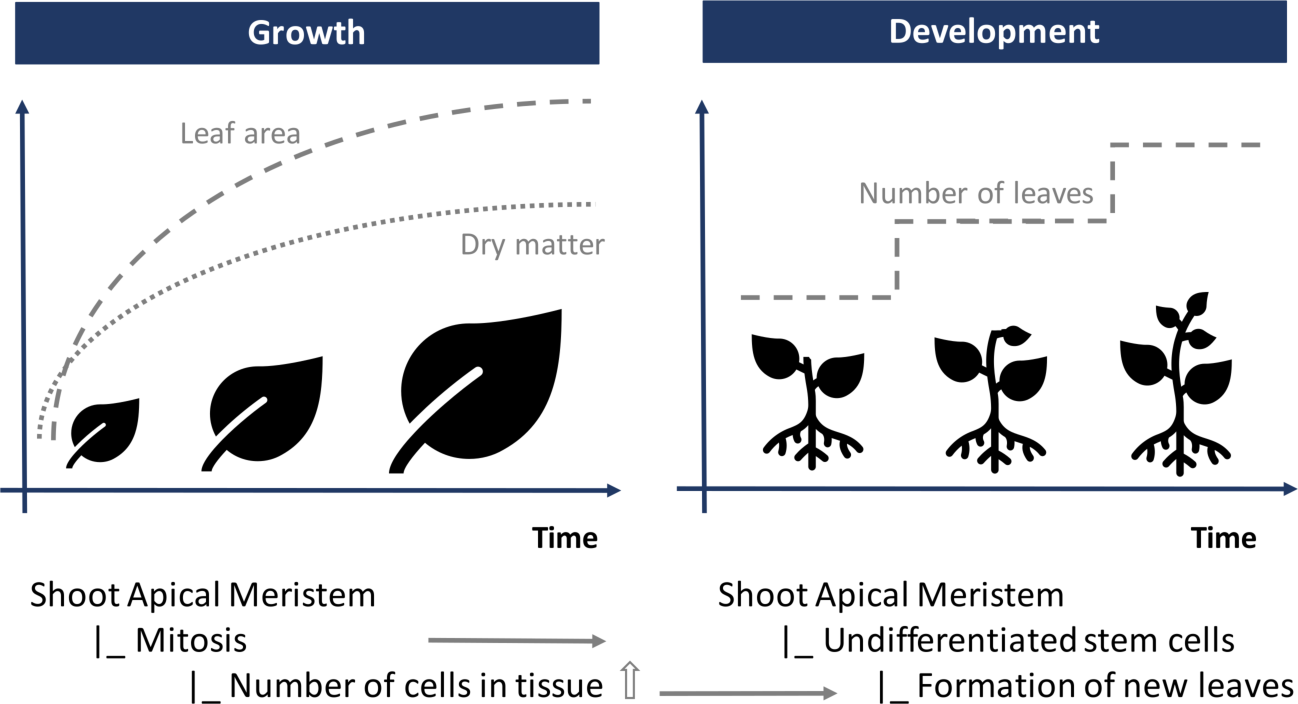
\includegraphics[width=\textwidth]{01-Introduction/img/growth_and_development.pdf}
    \caption{Illustrative example of leaf growth (left) by means of increasing leaf size and weight and plant development (right) by means of the appearance of new leaves from the main stem.}
    \label{fig:growth-development-biology}
\end{figure}

\subsection{Growth and development in winter wheat}

Winter wheat is an annual crop that uses the C3 photosynthetic pathway to fix atmospheric carbon. In the northern hemisphere, winter wheat is sown in the autumn (September to November in central Europe) and harvested in the summer (June to August) of the following year. Like all flowering plants, the development of winter wheat can be divided into a vegetative and a reproductive phase. To trigger this transistion, winter wheat requires vernalisation during the winter dormancy \citep{fedorov_photoperiodism_1976}, i.e. exposure to cold temperatures for a prolonged period.
Based on a growth-related perspective, \cite{kirby_analysis_1988} suggested to separate the growth and development process into three phases: The first phase consists of the formation of leaves and spikelets from the shoot apex. Following leaf development, tillers emerge from the axils of the leaves. This phases continues until the formation of the terminal spikelet and is followed by a vertical elongation of the stem and the ear. This second development stage finishes with the onset anthesis. In the third and last stage growth and development are mainly confined to the grains.

Building on the three phases suggested by \cite{kirby_analysis_1988}, the focus is on winter growth and development in the first and second stage, i.e., between the formation of tillers (tillering) and the full emergence of the inflorescence (end of heading). % TODO: why this period? -> second phase important for yield!

Figure \ref{fig:ww-growth-development} shows winter wheat growth and development between the tillering (\gls{BBCH} 20 macro-stage) and heading stage (\gls{BBCH} 50 marco-stage) depicting three growth-related traits and their trajectory with progressing phenology.

\gls{GCC} (orange line in Figure \ref{fig:ww-growth-development}) exhibits the highest dynamic during tillering and stem elongation. It increases from values around 10 to 20\% during early tillering up to 80 or 85\% at the beginning of booting. Afterwards, \gls{GCC} shows a slight decreasing tendency. % does this match with the literature

\gls{GLAI} (green line in Figure \ref{fig:ww-growth-development}) shows a slightly delayed pattern compared to GCC. is low during the tillering phase and increases steadily until reaching a peak during early heading. Typically, \gls{GLAI} values in winter wheat can take up to 8 $m^2$ $m^{-2}$. After heading, \gls{GLAI} decreases as the onset of senescence means a decrease in chlorophyll.

Dry biomass is the only trait out of the three that shows a continuous increase from tillering to heading (purple line in Figure \ref{fig:ww-growth-development}).

\begin{figure}[H]
    \centering
    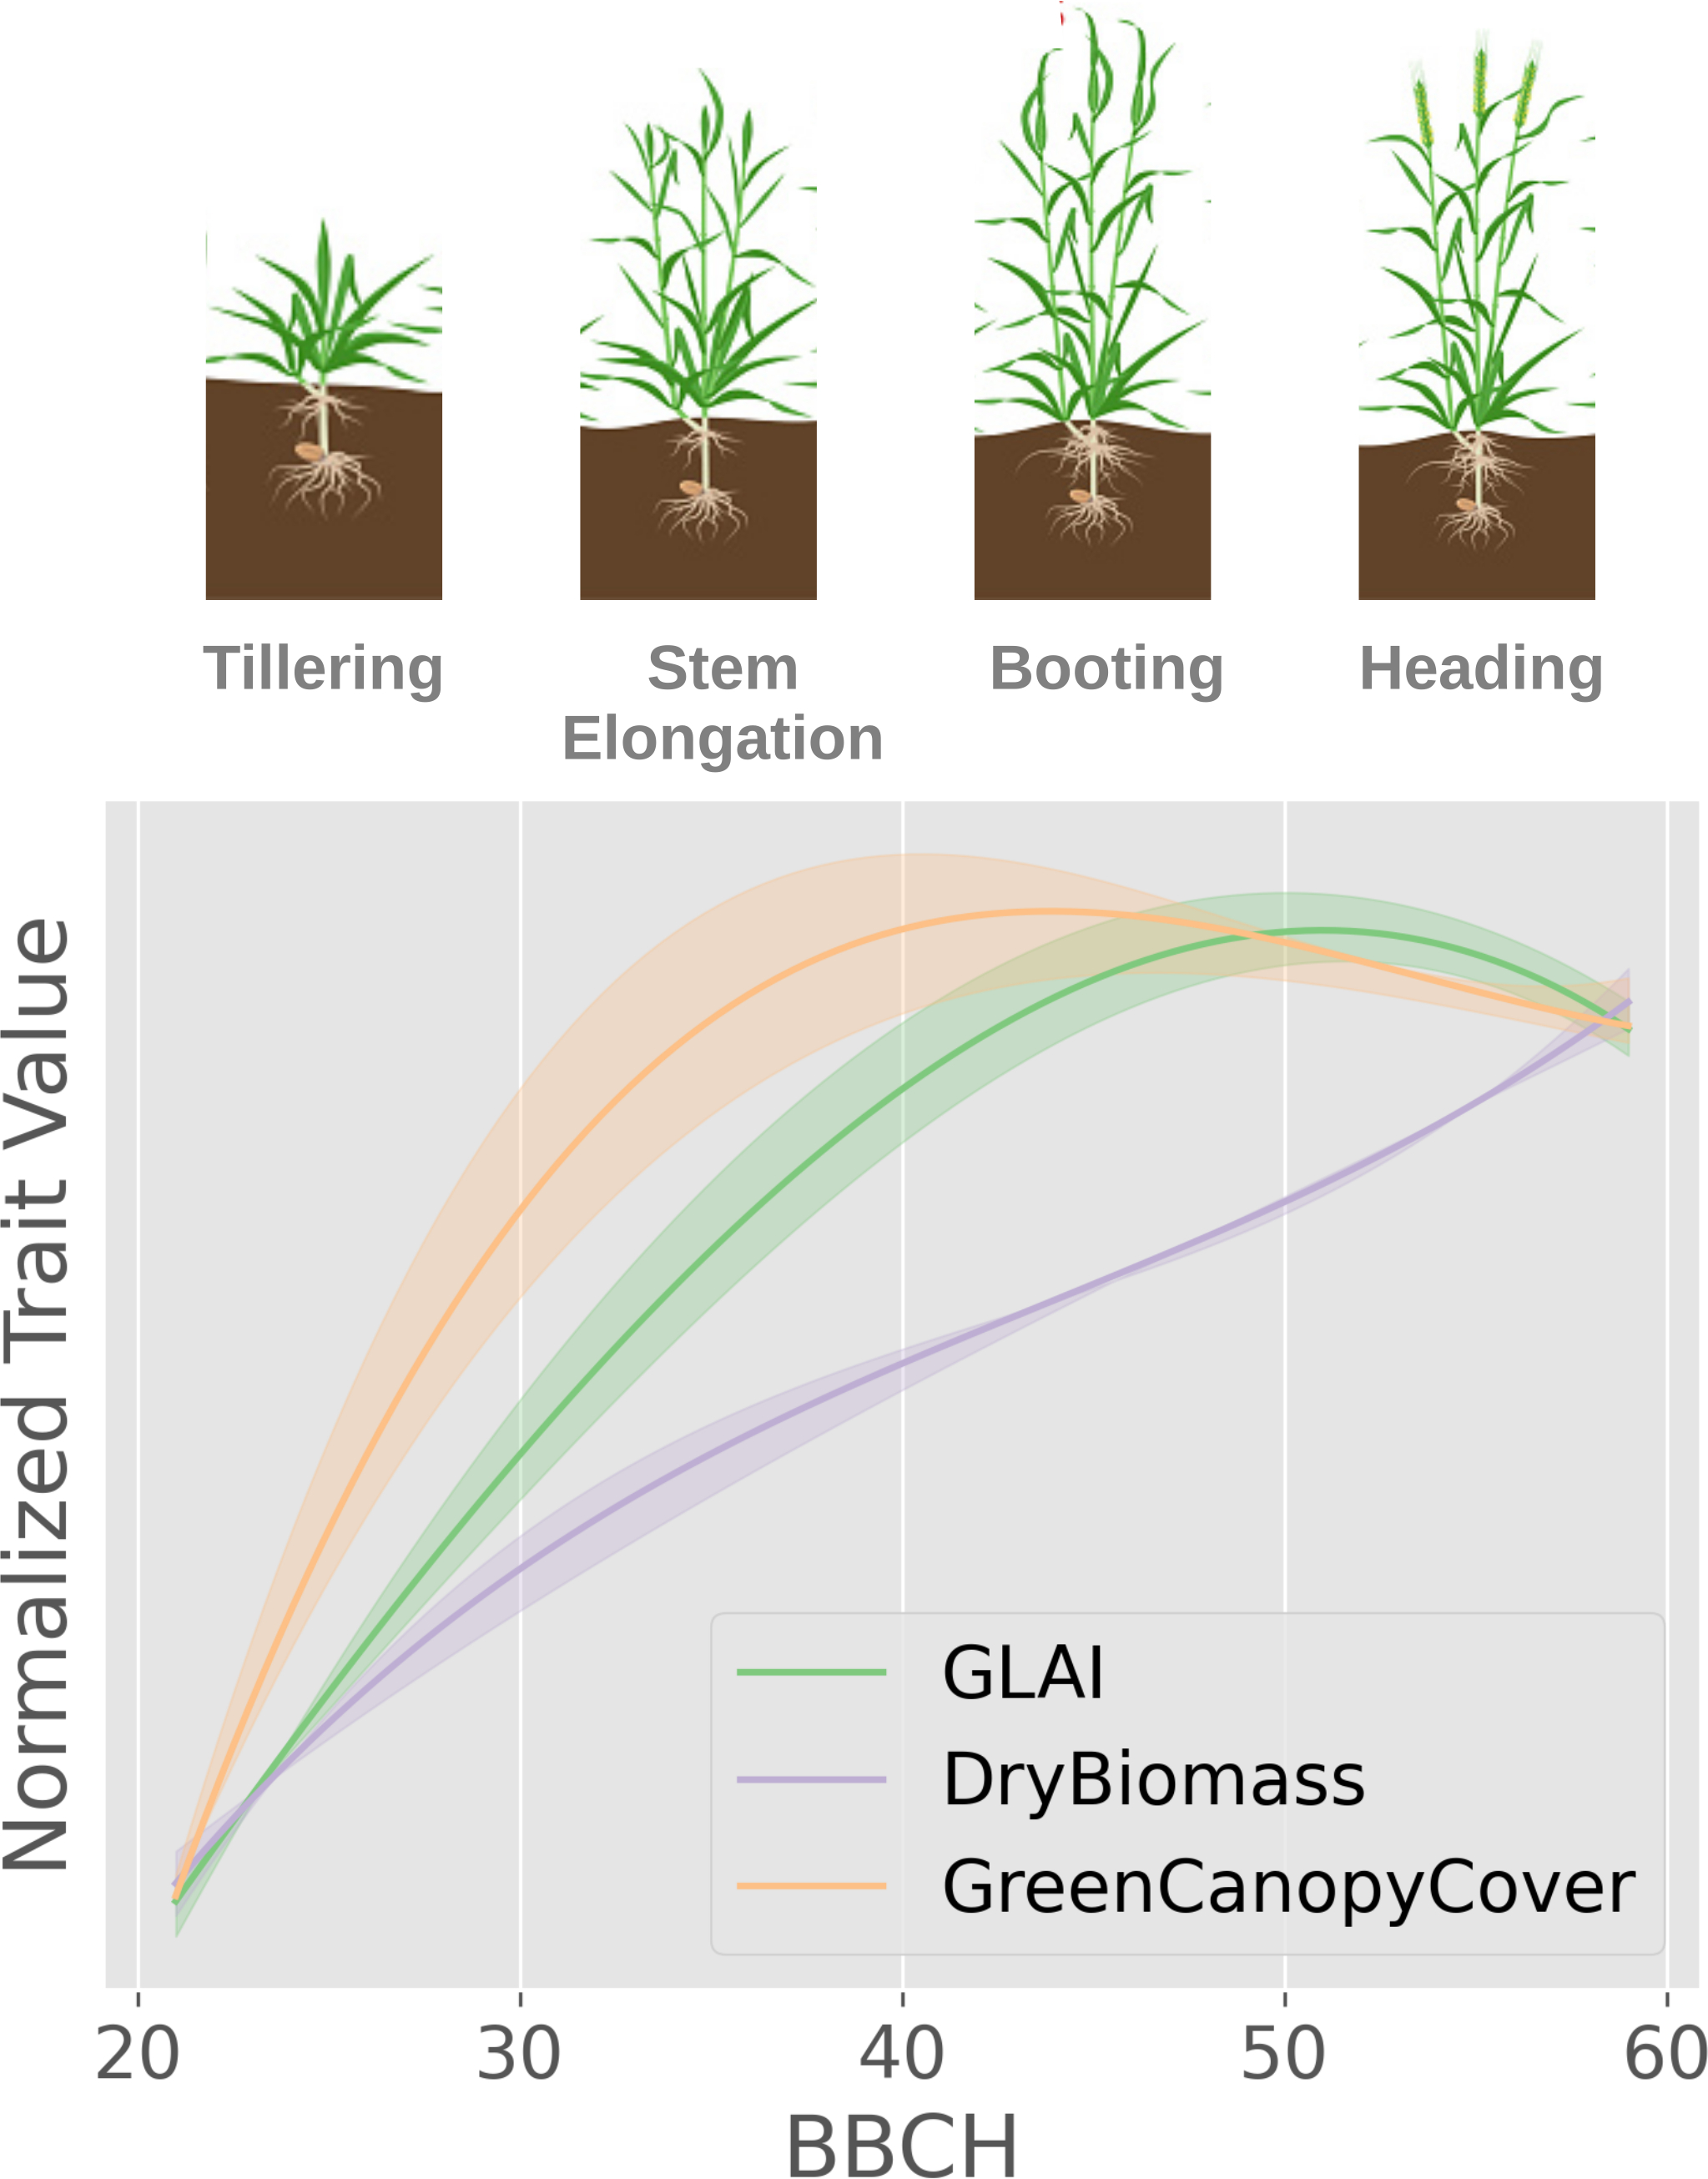
\includegraphics[width=\textwidth]{01-Introduction/img/figure_growth_and_development.jpeg}
    \caption{Growth and development in winter wheat between tillering and heading. The growth-related traits green leaf area index (GLAI, green), dry biomass (purple), and green canopy cover (orange) are plotted along the phenology axis expressed as BBCH growth stages. The trait values have been normalized between 0 and 1 to allow for a direct comparison.}
    \label{fig:ww-growth-development}
\end{figure}


\subsection{Field phenotyping, remote sensing and earth observation}

A key challenge is that the traits used in field phenotyping and remote sensing are often different and not necessarily compatible or interchangeable. Traits in field phenotyping often follow a physiological perspective on plant growth, such as \gls{DRC}s, while remotely sensed traits are often based on the ``traits-are-what-we-can-see'' principle, i.e. they are mostly spectral in nature, such as spectral indices \cite{bannari_review_1995} or absorption integrals \citep[for example]{wocher_rtm-based_2020}. As a result, coupling models from field phenotyping, such as complex mechanistic crop models and \gls{RTM} used in remote sensing, remains a challenge as model parameters are often incompatible, although some progress has been made \citep[for example]{thorp_estimating_2012}. There are also some terms that are defined or understood differently. For example, when the field phenotyping community refers to ``phenology'', they usually mean the timing of physiologically relevant transition phases in crop development, such as the onset of stem elongation in wheat. In the remote sensing community, however, ``phenology'' often refers to a change in spectral properties of crops, such as the increase in \gls{NDVI} after winter dormancy \citep{de_beurs_land_2004}.

% two disciplines that have similar aims but different approaches
% work on different scales, use different traits
% phenotyping traits: biological, physiological perspective
% remote sensing traits: focus on what we can see
% define EO as an umbrella term that might be better suited

% current methods in field phenotyping and RS
% highlight the missing link between field phenotyping and RS

\section{Objectives and research questions}

% How can we bridge field phenotyping and remote sensing using an EO approach?
% Can a combined approach out-perform "traditional" RS approaches?
% What are the (current) limitations and next steps and missing parts?

\section{Structure of the thesis}

This thesis is structured in six chapters excluding the Introduction.
